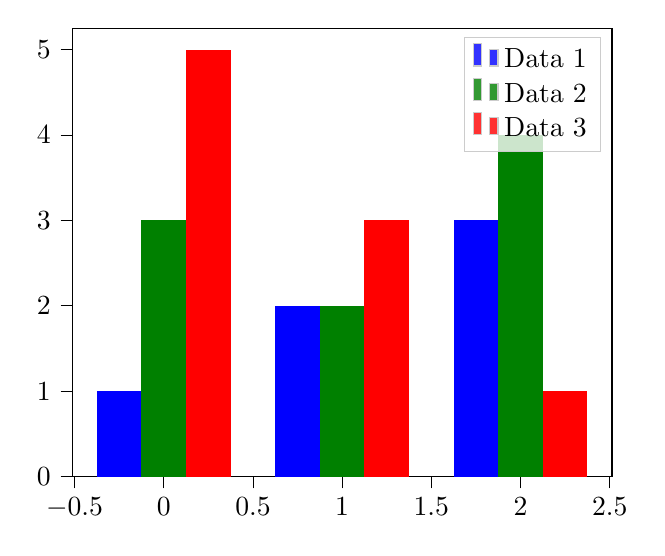
\begin{tikzpicture}

\begin{axis}[
legend cell align={left},
legend style={fill opacity=0.8, draw opacity=1, text opacity=1, draw=white!80!black},
tick align=outside,
tick pos=left,
x grid style={white!69.019608!black},
xmin=-0.5125, xmax=2.5125,
xtick style={color=black},
y grid style={white!69.019608!black},
ymin=0, ymax=5.25,
ytick style={color=black}
]
\draw[draw=none,fill=blue] (axis cs:-0.375,0) rectangle (axis cs:-0.125,1);
\addlegendimage{ybar,ybar legend,draw=none,fill=blue};
\addlegendentry{Data 1}

\draw[draw=none,fill=blue] (axis cs:0.625,0) rectangle (axis cs:0.875,2);
\draw[draw=none,fill=blue] (axis cs:1.625,0) rectangle (axis cs:1.875,3);
\draw[draw=none,fill=green!50!black] (axis cs:-0.125,0) rectangle (axis cs:0.125,3);
\addlegendimage{ybar,ybar legend,draw=none,fill=green!50!black};
\addlegendentry{Data 2}

\draw[draw=none,fill=green!50!black] (axis cs:0.875,0) rectangle (axis cs:1.125,2);
\draw[draw=none,fill=green!50!black] (axis cs:1.875,0) rectangle (axis cs:2.125,4);
\draw[draw=none,fill=red] (axis cs:0.125,0) rectangle (axis cs:0.375,5);
\addlegendimage{ybar,ybar legend,draw=none,fill=red};
\addlegendentry{Data 3}

\draw[draw=none,fill=red] (axis cs:1.125,0) rectangle (axis cs:1.375,3);
\draw[draw=none,fill=red] (axis cs:2.125,0) rectangle (axis cs:2.375,1);
\end{axis}

\end{tikzpicture}
